\chapter{系统架构设计}\label{chapter:architecture}
在第\ref{chapter:def}章定义了要解决的问题,并确定了实验的有关假设之后,本章我
来说明分布式二级哈希表的系统架构设计,而在第\ref{chapter:implementation}章中将
详细介绍系统各模块的实现细节。

对于像分布式二级哈希表这样的分布式存储系统,需要解决的关键问题主要包括以下几
点:
\begin{enumerate}
  \item 数据在集群中的单个结点上是如何存储的?
  \item 如何知道集群中哪些服务器结点当前是正常运行的?哪些已经发生了故障无法响
  应?进一步的,如果有结点发生了故障,那么是什么类型的故障?是因为系统负荷过大
  暂时无法响应,还是服务器程序崩溃或者系统故障需要重新启动,亦或是硬盘错误本地
  数据无法恢复?
  \item 数据在不同存储节点上是如何分配的?数据是如何存为多个副本的?给定索引如
  何确定数据存放在哪台(些)服务器上?
  \item 如何保证不同副本的数据一致性?
\end{enumerate}
分布式二级哈希表基于一些经典技术,在保证效率的前提下解决了这些问题,其架构如图
\ref{figure:architecture}所示。
\begin{figure}[htb]
  \centering
  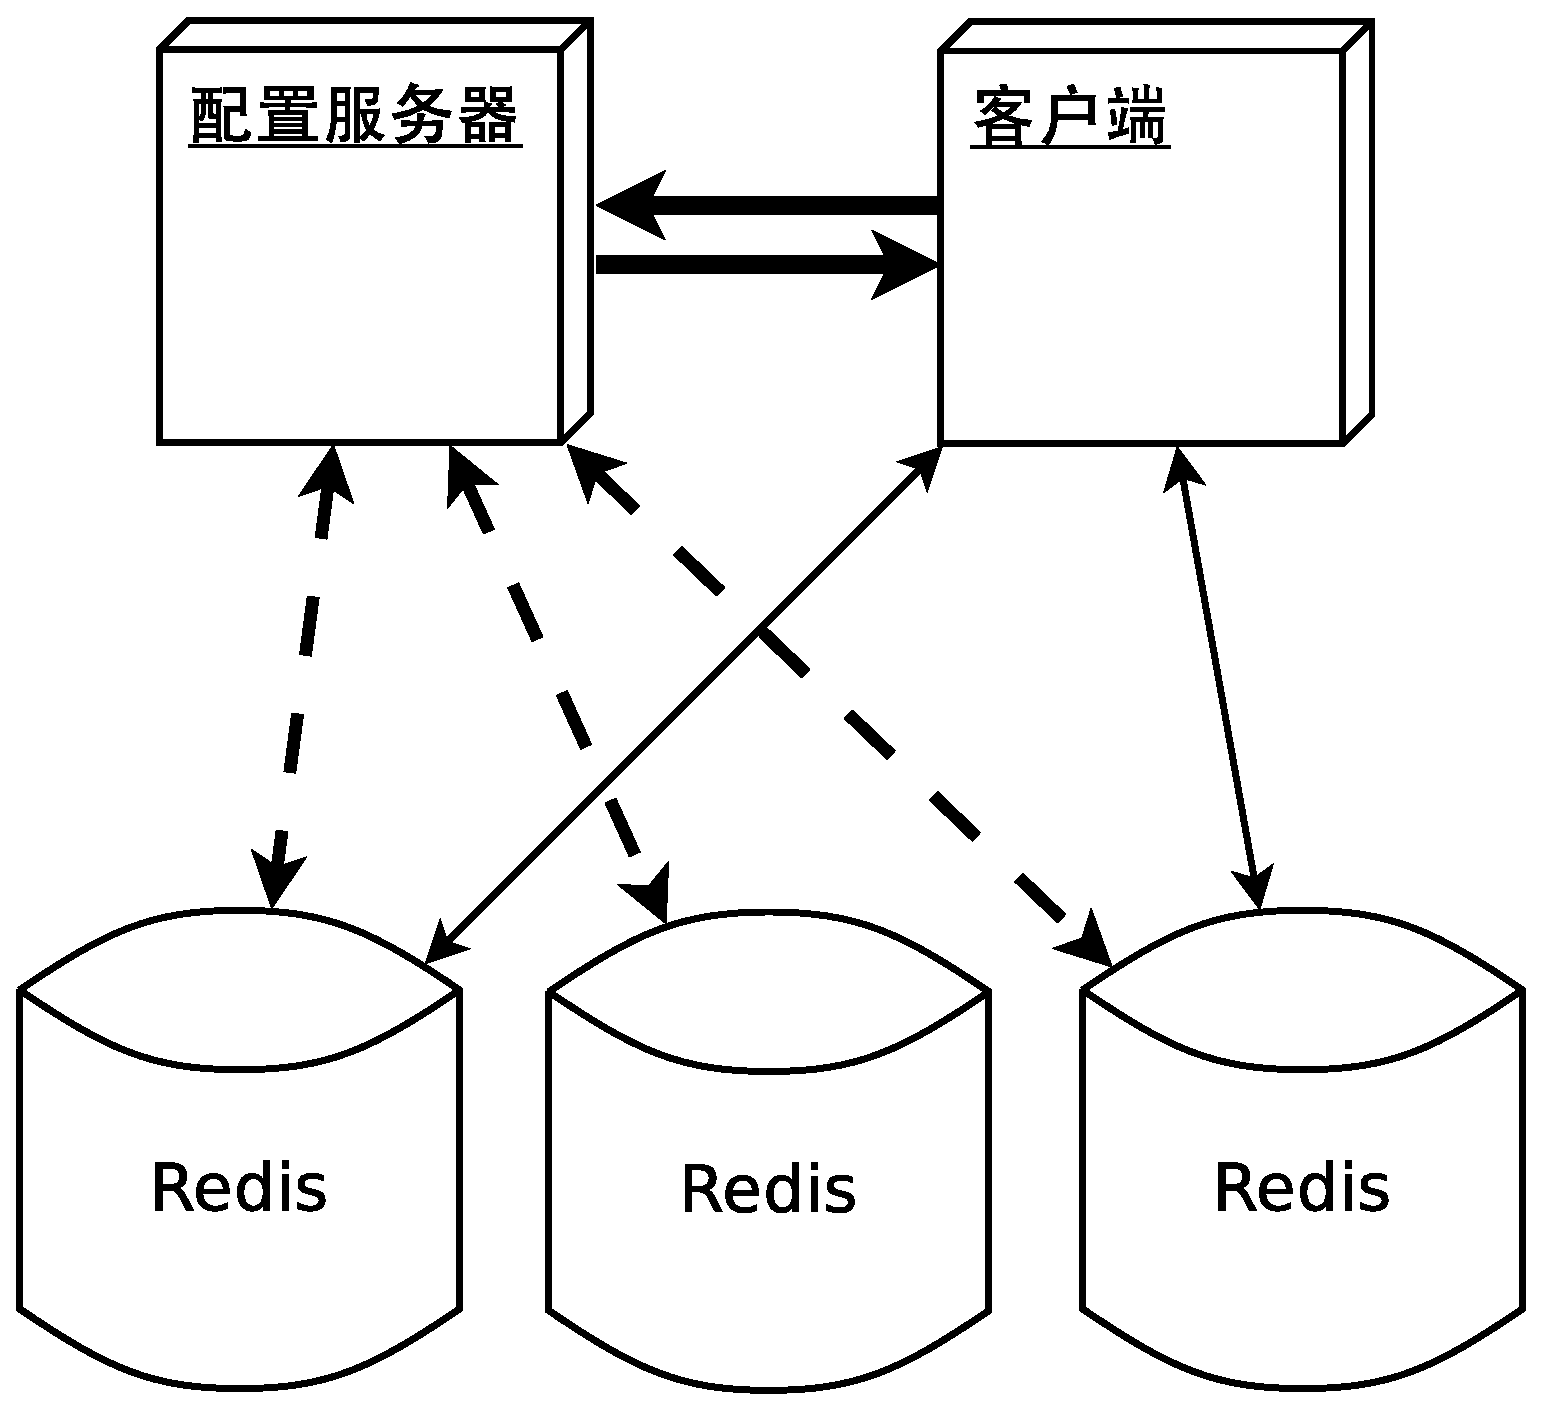
\includegraphics[width=0.8\linewidth]{architecture}
  \caption[分布式二级哈希表系统架构]{分布式二级哈希表系统架构。集群中设置一台
  配置服务器,与各节点进行心跳通信(虚线箭头),并且实现一致性哈希算法。上层应
  用嵌入客户端库代码,调用其中提供的接口函数,首先通过远程过程调用(粗实线箭
  头)从配置服务器获取某个bucketID对应的一系列存储服务器的地址,再遵照协议与这
  些服务器上的Redis进程进行socket通信(细实线箭头),完成相应操作。服务器集群中
  每个存储节点上运行一个Redis服务器进程。}
  \label{figure:architecture}
\end{figure}

集群中有一台特殊的配置服务器,通过与集群中其他的存储节点进行心跳通信,来确定当
前有哪些机器在正常运行。当前的系统设计不区分不同的故障类型,当配置服务器在一段
时限内与某存储服务器心跳通信失败,认为该服务器发生了错误,之后的操作不再涉及该
服务器。由于数据有多份副本,信息不会丢失。配置服务器的另一个功能是实现了一致性
哈希,对于某个特定的目标数据,根据它的bucketID,配置服务器负责指定多个服务器结
点存放该数据,并维护该信息,从而实现了数据的分配和备份。在第
\ref{subsection:consistent}小节我将详细介绍一致性哈希算法。

分布式二级哈希表提供了一个客户端库,里面包含表\ref{table:api}罗列的接口函数供
上层应用调用,上层应用需要嵌入客户端库代码。当上层应用发起请求时,客户端首先通
过远程过程调用\footnote{http://en.wikipedia.org/wiki/Remote\_procedure\_call}
从配置服务器获取存放着该数据的多台目标服务器的IP地址,然后按照Redis规定的协
议,通过socket通信
\footnote{http://en.wikipedia.org/wiki/Computer\_network\_programming}同时向这
些目标服务器发起请求并接收应答。为了提高系统的运行效率,客户端还做了多项优化,
并且通过线程池实现了异步请求,详见第\ref{section:client}节。

在存储服务器集群中的每个结点上,都运行着一个Redis存储服务器进程。Redis是一个开
源本地哈希表项目。与一般的哈希表不同,Redis的值类型除了可以是一般的字符串,还
可以是列表、集合甚至哈希。所以Redis实际上已经解决了本地二级哈希的问题。Redis的
另一个优点是它在应用层实现了一个虚拟存储层,将所有数据存于内存和应用层虚存中大
大提高了系统运行效率。同时,Redis是基于日志的事务型存储系统,保证了操作的原子
性,并具备一定的容错能力。有关Redis的更多细节我将在第\ref{section:redis}节做进
一步介绍。

分布式哈希表的架构设计与主流分布式存储系统有很多相似之处,其优点显而易见。
\begin{enumerate}
  \item 数据被分配到多台存储服务器之上,包含多个副本,数据的分配和备份采用一致
  性哈希算法。系统中包含的单个存储单元越多,单个存储单元的容量越大,系统的总存
  储容量就越大。数据分别存放在多台存储服务器上,提升了系统的运行效率。单个存储
  单元的硬盘读写速率和网络带宽有一个上限,如果客户端能够同时与多台服务器进行数
  据通信,便提高了单位时间内的数据交换速率,使得系统的总体运行效率大大提升。另
  一方面,由于系统对数据进行了备份,在不同的存储结点上保留了多个副本,即便某个
  存储节点由于发生了灾难性的故障导致数据永久丢失,系统仍可以通过该数据在其他正
  常运转的服务器上的副本将该数据恢复,这大大增强了系统的容错能力。一致性哈希算
  法作为经典的数据分配算法,被很多著名的分布式存储系统所采用。
  \cite{hastorun2007dynamo}由于已知分布式二级哈希表的集群规模在几十台服务器左
  右,机器故障并不会频繁发生,当前的系统进行了数据备份,不支持存储结点动态加入
  和离开集群。但是一致性哈希算法自诞生之日起,受到青睐的原因之一在于它很好的支
  持了系统中存储结点的动态变化,所以分布式二级哈希表具备实现该功能的潜能。事实
  上,只要在当前系统上添加一个后台数据迁移模块,即可实现存储节点的动态添加和移
  除功能。
  \item 集群中有一台特殊的配置服务器,监控集群中所有存储结点是否运转正常,并实
  现一致性哈希算法。配置服务器与集群中各存储结点进行心跳通信,了解各存储服务器
  的运转情况。相比传输的数据,心跳信息所占用的网络带宽和消耗的系统计算资源基本
  可以忽略不计。因而使用单一的服务器维护控制信息对系统性能造成的影响是微乎其微
  的。另一方面,集中管理控制信息与非集中策略相比,不用考虑信息同步问题,不仅简
  化了系统实现,也方便客户端获得此信息。此外,当前的系统架构设计假设配置服务器
  不会发生系统故障。如果确实需要解决这个问题,只需要再安置一台配置服务器,存储
  控制信息的副本,并定期从主配置服务器获取信息更新。一旦主配置服务器发生系统故
  障,该替补配置服务器立刻接替其工作,继承原配置服务器的属性
  \footnote{如IP地址。},即可实现配置服务器的无缝替换。
  \item 上层应用需要嵌入分布式二级哈希表系统提供的客户端库代码,以调用其中提供
  的接口函数。这种机制在一定程度上影响了系统的易用性,优点是客户端和上层应用之
  间不需要进行网络通信。另一种机制使得上层应用不必嵌入任何系统代码,而是按照系
  统规定的协议与任何一台存储结点或入口服务器通信,再由此机器经过一次路由选择将
  该请求发送至目标服务器,操作完成后再将返回值传回上层应用。缺点是需要附加一次
  网络通信,对网络带宽和操作延迟提出了更高的要求。在
  \onlinecite{hastorun2007dynamo}中详细讨论了两种机制的优劣和适用场合。由于分
  布式二级哈希表在设计之初就本着尽量提高系统运行效率的原则,而其所支撑的上层应
  用目前都是由我们自己设计和实现的工程,所以分布式二级哈希表采用了第一种机制实
  现客户端。
  \item 客户端通过远程过程调用从配置服务器获取存储服务器的IP地址,再与这些存储
  服务器通过socket通信进行实际的数据传输。在分布式二级哈希表系统中,由于控制信
  息只包含目标存储服务器的IP地址,一次操作需要获取的控制信息只有10字节左右。所
  以尽管整个系统只有一台配置服务器提供控制信息,该服务器依然可以承担相应的负
  担。另一方面,由于实际存储的一份数据最大有1MB,因此实际的数据传输直接在客户
  端和相应的存储服务器之间进行。这种数据分散传输的机制充分利用了各个存储服务器
  的网络带宽和硬盘读写能力,不会由于出现某个瓶颈,而造成整个系统的运行效率降
  低,因而这种设计被很多著名的分布式存储系统所采纳。\cite{ghemawat2003google}
\end{enumerate}
